% Copyright (C)  2015  Alexander Jankowski, Philipp Hacker.
% Permission is granted to copy, distribute and/or modify this document
% under the terms of the GNU Free Documentation License, Version 1.3
% or any later version published by the Free Software Foundation;
% with no Invariant Sections, no Front-Cover Texts, and no Back-Cover Texts.
% The lincense itself can be found at <https://www.gnu.org/licenses/fdl-1.3>.

\documentclass[numbers=noenddot,a4paper]{scrartcl}

\usepackage{ifoddpage}
\usepackage[infoshow]{tabularx}
\usepackage{fancyhdr}
\usepackage[greek,ngerman]{babel}
\usepackage[T1]{fontenc}
\usepackage[utf8]{inputenc}
\usepackage{libertine}
\usepackage{ziffer}
\usepackage{graphicx}
\usepackage{units}
\usepackage[infoshow]{tabularx}
\usepackage[all]{xy}
\usepackage{amsmath}
\usepackage{amssymb}
\usepackage{wrapfig}
\usepackage{upgreek}
\usepackage{esint}
\usepackage{float}
\usepackage[font=small,labelfont=bf]{caption}
\usepackage{subcaption}
\usepackage{lscape}
\usepackage[backref=page]{hyperref}
\usepackage{cleveref}
\usepackage{csquotes}

\renewcommand{\headrulewidth}{0.1pt}
\renewcommand{\footrulewidth}{0.1pt}
\newcommand{\name}{\text{Philipp Hacker}} %TODO Name des Protokollanten eintragen

\renewcaptionname{ngerman}{\figurename}{Abb. }
\renewcaptionname{ngerman}{\tablename}{Tab.}

\setlength{\parindent}{0pt}

\newcommand{\nummat}[1]{\left[\text{#1}\right]}
\newcommand{\num}[1]{$\left[\text{#1}\right]$}
\newcommand{\degree}{^\circ}
\newcommand{\diff}{\textnormal{d}}
\newcommand{\tenpo}[1]{ 10^{#1}}
\newcommand{\greek}[1]{\greektext#1\latintext}
\newcommand{\ix}[1]{_\text{#1}}
\newcommand{\imag}{\mathbf{i}}
\newcommand{\tilt}[1]{\textit{#1}}
\newcommand{\grad}[1]{\textit{grad}\left(#1\right)}
\newcommand{\divergenz}[1]{\textit{div}\left(#1\right)}
\newcommand{\euler}{\mathnormal{e}}
\newcommand{\fett}[1]{\textbf{#1}}
\newcommand{\einnup}{\hspace{0.2cm}}
\newcommand{\einnum}{\hspace{-0.2cm}}
\newcommand{\zentriert}[1]{\begin{center}#1\end{center}}

\title{Protokoll: Positronen und Koinzidenz-Messungen} %TODO Name des Versuchs eintragen
\author{Alexander Jankowski, Philipp Hacker}
\date{\today}
\pagestyle{fancy}
\fancyhead[C]{\thepage}
\fancyhead[R]{\name}
\fancyfoot[C]{\thepage}
\fancyhead[L]{Abschnitt \thesection}

\begin{document}
	\maketitle
	\begin{center}
		Betreuer: Gerrit Marx\\ %TODO Name des Betreuers eintragen
		Versuchsdatum: 21./22./23.10.2015\\ %TODO Datum des Versuchs eintragen
		\begin{table}[h]
			\centering
			Note: %TODO Gute Note erhalten :)
			\begin{tabularx}{1.5cm}{|X|}
				\hline \\ \\
				\hline
			\end{tabularx}
		\end{table}
	\end{center}
	\vspace*{\fill}
	\tableofcontents
	\vfill
	\newpage
	\section{Motivation}

	In diesem Versuch geht es um den Aufbau, die Kalibrierung und Anwendung von Hochpräzisions-Elektronik auf die Lebensdauermessung von Positronen. Einerseits galt es hierbei Einblick in die unterschiedlichen Wechselwirkungsarten von $\textbf{e}^+$ bzw. $\beta^+$-Strahlung mit Materie zu erhalten, und andererseits die Kunstgriffe und Bestandteile von schneller Zeit-Messtechnik kennen zu lernen. Insbesondere die Idee der Beobachtung und Interpretation atomar koinzidenter Ereignisse mit Hilfe von geeigneten Konstruktionen wurde hierbei näher gebracht. Ob, wann und in welcher Weise zwei Quanten einen gemeinsamen Ursprung haben bzw. in Zusammenhang stehen kann eine Fragestellung zu diesem Experiment sein.

	\newpage
	\section{Physikalische Grundlagen}

		\subsection{Erzeugung und Vernichtung von Positronen}\label{subsec:psoitronen}
	
			\begin{wrapfigure}{r}{0.55\textwidth}
				
\includegraphics[width=0.55\textwidth,height=0.5\textwidth]{zerfallsschema.png}
				\caption{Schema eines, von einem $\beta^+$-Zerfall erzeugten Positrons (aus \cite{Augsten08}). Im Bereich der "`Thermalization"' kommt es zu Stößen/Streuung des Positrons in Materie.}
				\label{img:zerfall}
			\end{wrapfigure}
	
			Das Positron ist ein stabiles Lepton mit der Leptonenzahl $L=-1$, dem Spin $s=\frac{1}{2}$ und das Anti-Teilchen des Elektrons. Somit gehört es, dem Standardmodell zur Folge, zu den Elementarteilchen und damit den grundlegenden Bausteinen der Materie. Es wird durch das Symbol $\textbf{e}^+$ ausgedrückt. Dessen Ladung ist die entgegensetzte zum Elektron $q=1\cdot\text{e}=\unit[1,602 176462(63)\cdot\tenpo{-19}]{C}$ (ebenso magnetisches Moment), seine Masse ist gleich der des $\textbf{e}^-$ $m_{\textbf{e}^+}=\unit[9,10938188(72)\cdot\tenpo{-31}]{kg}$ und auch in allen anderen Eigenschaften stimmen die beiden Teilchen überein. Es wurde 1928 vom Nobelpreisträger \tilt{Paul M. Dirac} vorhergesagt und erstmal 1932 von \tilt{Carl David Anderson} in der kosmischen Strahlung nachgewiesen. Das Positron tritt also u.a. beim Zerfall positiver Myonen in der Atmosphäre, dem $\beta^+$-Zerfall mit der Form
			
			\begin{align}
				^{X}_{Z}A \rightarrow ^{X}_{Z-1}B+\textbf{e}^{+}+\nu\ix{e}+\gamma
			\end{align}
	
			oder bei hochenergetischen Stoßprozessen bzw. der Proton-Proton-Wechselwirkung.\\
			Treffen Teilchen und Anti-Teilchen aufeinander ($\textbf{e}^+$ und $\textbf{e}^-$), so kommt es zu deren Wechselwirkung in Form der Bildung des \tilt{Positroniums} - sozusagen dem "`Anti-Atom"' zum Wasserstoff, welches jedoch sehr kurzlebig ist. Das Positronium besteht demnach im "`Kern"' aus einem Positron und dem, auf einer Kreisbahn umlaufenden Elektron. Je nach Spin-Einstellung der beiden Fermionen - parallel als \tilt{ortho-} oder anti-parallel als \tilt{para-Positronium} - ändert sich die Lebensdauer des Pseudo-Atoms: etwa $\unit[\tenpo{-7}]{s}$ bzw. $\unit[\tenpo{-9}]{s}$. Sind die Streupartner zu schnell oder langsam (der Wirkungsquerschnitt ist stark energieabhängig), kommt es, ohne Ausbildung und Zerfall eines gebundenen Zustandes vorher, zur Paarvernichtung. Dabei \tilt{annihilieren} sich Elektron und Positron unter Emission von 2 Photonen mit Gesamtenergie der kinetischen Energie beider Teilchen und deren Ruhemassen. Unter Voraussetzung, dass das Elektron stationär und das Positron stark verlangsamt ist, ergibt sich eine Photonen-Energie von $\unit[511]{keV}$. Der Winkel, unter welchen diese beiden sich auseinander bewegen, wird, mit den selben Annahmen, zu $\sim\unit[180]{\degree}$.\\
			Die Erzeugung von Positronen in diesem Versuch erfolgt über eine $^{22}Na$-Quelle, die über einen $\beta^+$-Zerfall in $^{22}Ne$ übergeht. Das entsprechende Schema zeigt \autoref{img:schemana22}. Aufgrund der langen Halbwertszeit des Natriums sind dabei moderate Zählraten zu erwarten.\\
			Zusammen mit dem Positron und Elektron-Neutrino entsteht auch ein hochenergetisches "`Start"'-Photon - mit etwa $\unit[1,274]{MeV}$ - aus der Abregung eines dazwischen gelegenen Niveaus. Die Lebensdauer dessen liegt außerhalb des Bereiches der zu erwartenden Halbwertszeiten der Positronen, weshalb diese Emission als quasi-instantan mit der des $\textbf{e}^+$ zusammen angenommen werden kann. Dieser Fakt und der Energieunterschied in den Photonen von Annihilation und Zerfall eröffnen die Möglichkeit der Koinzidenzmessung (siehe \ref{subsec:koinz}).\\

							\begin{figure}[t]
								\centering
								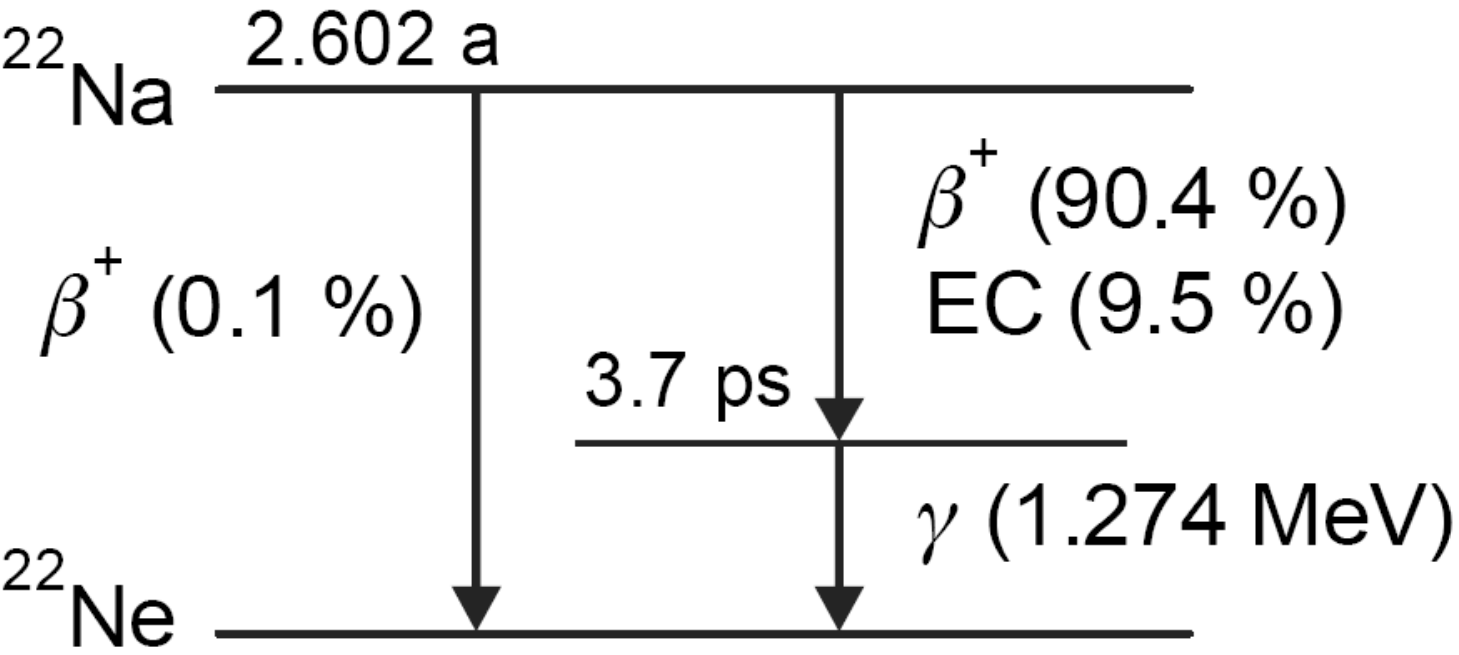
\includegraphics[width=0.5\textwidth]{termschema.png}
								\caption{Niveau-Darstellung des $\beta^+$-Zerfalls von $^{22}Na$ unter Aussendung eines zusätzlichen $\unit[1,274]{MeV}$-Photons. Angegeben sind auch die Halbwertszeit des Natriums und die Lebensdauer des Zustandes zur Erzeugung des "`Start"'-Photons (aus \cite{Augsten08}).}
								\label{img:schemana22}
							\end{figure}

			Einen grundlegenden, experimentellen Zusammenhang von Erzeugung, Vernichtung und Energiespektrum dieses Versuchs zeigt \ref{img:zerfall}. Da der Emissionswinkel zwischen den "`Stop"'-Photonen $\sim\unit[180]{\degree}$ beträgt - weswegen eine gedachte Gerade zwischen diesen gezogen werden kann -, können 2 gegenüberliegende Detektoren, deren Fenster die sogenannte \tilt{Koinzidenz-Linie} überdecken, diese aufnehmen. Dieser Prozess ist über den gesamten Raumwinkel gleichverteilt. Genauere Prinzipien der Messtechnik werden im nächsten Abschnitt \ref{subsec:koinz} beschrieben.\\
			Da ein emittiertes Positron von seinem Entstehungsort bis zu seiner Annihilation eine endliche Wegstrecke zurücklegt und dessen Lebenszeit nicht $\unit[0]{s}$ beträgt, ist es naheliegend, vor der Paarvernichtung eine Streuung innerhalb von Materie anzunehmen. Des weiteren kann man dies auch als Forderung für die beobachtete Ausbildung von Positronium ansehen: das $\textbf{e}^+$ muss erst verlangsamt werden, bevor es einen gebundenen Zustand eingehen kann. Das Kriterium dafür ist, dass die restliche kinetische Energie des Positrons in der Größenordnung der thermischen Anregungen innerhalb des vorliegenden Festkörpers ist \cite{Augsten08}.\\
			Damit moduliert die Zeitspanne von dem Ereignis des Zerfalls bis zur Detektion der Photonen aus der Vernichtung. Sie wird zu einer Funktion der Materie- bzw. Elektronendichte $n\ix{-}\left(\vec{r}\right)$. Mit der Positronendichte $n\ix{+}\left(\vec{r}\right)$, dem klass. Elektronenradius $r\ix{0}$ und der Lichtgeschwindigkeit in dem vorliegenden Medium $c$ ergibt sich für die Annihilationsrate $\lambda$ bzw. die Lebensdauer $\tau$

				\begin{align}
					\lambda=\frac{1}{\tau}=\pi r\ix{0}^{2}c\int n\ix{+}\left(\vec{r}\right)\left(1+\frac{\Delta n\ix{-}\left(\vec{r}\right)}{n\ix{-}\left(\vec{r}\right)}\right)\diff \vec{r} \,\, .
				\end{align}

			Dabei ist $\Delta n\ix{+}\left(\vec{r}\right)$ die durch das Positron hervorgerufene Pertubation von $n\ix{-}$ an seinem Ort $\vec{r}$. Die Messung der Lebensdauer kann also zur Bestimmung von lokalen Elektronendichten genutzt werden.\\
			Schließlich erfahren auch die am Ort der Vernichtung erzeugten Photonen Streuung und Abbremsung. Idealer Weise detektiert man zwei Teilchen mit der Energie von $\unit[511]{keV}$, jedoch sieht die Praxis anders aus: das Spektrum der aufgenommenen Photonen reicht von \mbox{$\unit[511-0]{keV}$}. Betrachtet man ein vollständiges Energiespektrum (Intensität über Energie) so beeinflussen die sog. \tilt{Compton}-Kanten im Diagramm das Bild der Messung stärker, als die Peaks der erwarteten Energien. Aufgrund des namensgebenden Compton-Effekts verändert sich die Wellenlänge der Photonen bei ihrer Wechselwirkung mit Materie bis zu einem kritischen Wert, der \tilt{Compton-Wellenlänge}, mit welcher natürlich eine Energie korrespondiert. Daher ist das Spektrum in 2 Bereiche - dem des Start-Photons aus der $^{22}Na$-Quelle und seiner Aufweichung bis zu $\lambda\ix{C}$ und analog dem der Stop-Photonen der Annihilation - zu unterteilen, was für den Abschnitt \ref{subsec:koinz} eine wichtige Rolle spielt. Zu dieser Unterscheidung kommt hinzu, dass das Positron/Positronium in verschiedenen Zuständen im Medium zerstrahlt: Defekten, Löchern, defektfreien Elektronenschalen, ortho- oder para-Positronium \dots . Deswegen setzt sich letztlich das Spektrum der Annihilations-Photonen aus mehreren Spezies $k$ von Ereignissen zusammen. Das Lebensdauerspektrum $T\left(t\right)$ geht über einen \tilt{Lambert-Beer}'schen Exponentialzusammenhang aus

			\begin{align}
				T\left(t\right)=\sum_{k}\frac{I\ix{k}}{\tau\ix{k}}\exp\left(\frac{-t}{\tau\ix{k}}\right)
			\end{align}

			hervor. Dieser Ausdruck ist darauf begründet, dass die Zahl der Photonen für die verschiedenen \tilt{Koinzidenzen}, welche für die Zeitmessung essentiell sind, einer exponentiellen Extinktion vor ihre Detektion folgen.

		\subsection{Start-Stop-Koinzidenzmessungen}\label{subsec:koinz}

			Wie bereits in \ref{subsec:psoitronen} erwähnt, benötigt man die Unterscheidung und Energie-aufgelöste Detektion von 2 $\gamma$-Quanten innerhalb einiger Nano- bzw. Pico-Sekunden. Damit sind enorme Anforderungen an die Empfindlichkeit und Geschwindigkeit der Messtechnik gestellt. Um diese zu erfüllen, bedient man sich einiger Tricks und komplizierter Elektronik.Das Startsignal wird als das, von der $Na$-Probe ausgesandte $\unit[1,274]{MeV}$-Photon angenommen (quasi-instantane Aussendung mit dem Positron). Der Stop-Puls sei \underline{\textbf{eines}} der beiden $\unit[511]{keV}$-Quanten der Annihilation.\\
			Auf gegenüberliegenden Seiten der $^{22}Na$-Probe befinden sich 2 Szintillationsschirme - Kristalle, in denen durch energiereiche Strahlung Lichtblitze aus Grundzustandsübergänge erzeugt werden -, an welche wiederum eine Photokathode folgt. Die Kristalle haben eine sehr geringe Totzeit, können also dicht aufeinander folgende Signale unterscheiden und eigenen sich daher gut für diese Untersuchung. Ein weiterer Vorteil ist, dass ab einer spezifischen Minimalenergie das Photoelektrische Signal proportional zur Energie der eingestrahlten Photonen ist. Damit erschließt sich eine Energieauflösung der erfassten $\gamma$-Quanten. Die Photokathode wandelt, die in den Szintillatoren durch die Photonen erzeugten Lichtsignale in einige Elektronen um. Ein Dynodensystem beschleunigt jene dann so, dass etwa $\tenpo{7}$ Sekundärelektronen pro Initialelektron entstehen. Ein zwischengeschalteter Verstäker (\tilt{amplifier}) soll für eine möglichst steile Signal-Flanke für die digitale Detektion sorgen.\\
			Der erhaltene Puls geht in einen sog. \tilt{constant-fraction-discriminator} (\textbf{CFD}). Dieser gibt, falls der Eingang eine bestimmte Schwelle überschreitet, ein logisches Signal mit fester Höhe und Breite aus. Um zu verhindern, dass gleichzeitige Signale mit unterschiedlichen Amplituden verschiedene Ergebnisse dieser Zeit-Auflösung erzeugen, verschiebt, staucht und invertiert der CFD (\tilt{konstant}) die Eingänge - demnach löst dieser den Null-Durchgang, welcher somit für alle Ereignisse gleich wird, auf \cite{TUDarmstadtPET}.\\
			Bisher erhält man aus einem Ereignis (Positronen-Erzeugung und Annihilation) 2 (maximal 3) Energie-aufgelöste - hierbei interessiert nur, ob es das Start- oder Stop-Photon war -, logische Rechteck-Pulse. Ein \tilt{time-to-amplitude-converter} (TAC) kann über die variierende Entladung von Kondensatoren an seinem "`Start"'- und "`Stop"'-Eingang die Zeit zwischen diesen Signalen in eine Spannungsspitze mit variabler Höhe umwandeln. Dieses korrespondiert dann mit der dazwischen verstrichenen Zeit.\\
			Um "`verschluckte"' Koninzidenzen oder falsche Zuordnungen von zeitnahen Emissionen/Annihilationen auszuschließen, schaltet man einen \tilt{delay} zwischen die Kanäle von Start und Stop am TAC, weil nicht festgelegt ist, welcher Detektor welches Event aufnimmt. Um dies zu verhindern, legt man zwischen Detektion und TAC-Stop-Kanal eine Delay-Box, welche über verschiedene Kabellängen einige Nano-Sekunden Verzögerung erzeugen kann.\\
			Mehrere \tilt{analog-to-digital-converter} (ADC) und ein \tilt{multichannel-analyzer} (MCA) konvertieren die Zeit-Signale in digitale Rechteck-Pulse, welche von dem MCA je nach Höhe (Lebensdauer) gespeichert und ausgegeben werden. Damit ist der Weg von, idealer Weise 2 koinzidenten $\gamma$-Quanten bis zu einer digitalen Auswertung gemacht. Fehlermöglichkeiten bestehen trotz der fortschrittlichen Technik: nicht-koinzidente Signale können einander zugeordnet werden (\tilt{trues}, \tilt{randoms}, \tilt{singles} usw., siehe \cite{Wiki:PET}), zusammengehörige Ereignisse liegen dennoch innerhalb der Totzeit der Elektronik, \dots . 

	\newpage
	\section{Durchführung}

		Wie es in \ref{subsec:koinz} beschrieben wurde, galt es den Versuch aufzubauen und entsprechend zu kalibrieren. Mit der Kenntnis aus diesem Abschnitt über die verwendete Elektronik vereinfacht sich diese Herleitung.\\
		Vorerst wurde sichergestellt, dass beide Detektoren mit Hilfe der Szintillatoren, Dynoden und \tilt{amplifier} ohne weitere Einschränkungen in etwa gleiche Spektren zeigen (Forderung, dass die Positronen-Emission und Annihilation isotrop war). Anschließend daran musste die Relation: Kanal-Energie festgelegt werden. Einhergehend damit war die Unterteilung des Spektrums in den Teil des Start-Photons aus der $\beta^+$-Quelle und den Vernichtungs-$\gamma$-Strahlen. \\
		Die Einstellung des CFD wurde danach vorgenommen - jeweilige Ergebnisse wurden mit einem Oszilloskop beobachtet. Ein weiter wichtiger schritt war die Kalibrierung der Kanäle des MCA mit den ADC und der Delay-Box: mit Hilfe der festen Zeitverschiebungen konnten die Kanäle des MCA leicht nach der Zeit aufgelöst werden.\\
		Wurde dies getan, konnten die jeweiligen Messungen beginnen. Dafür war es lediglich notwendig die Kalibrierten Start-/Stop-Kanäle des TAC (zwischengeschalteten \tilt{delay}) mit den Signalen der CFD zu versorgen und somit Messergebnisse zu erhalten. Dessen Ausgang an den MCA angeschlossen, ergab sich am PC ein ähnliches Bild wie in \autoref{img:beispielspektrum}. Den endgültigen Aufbau zeit \autoref{img:aufbau}. Für eine $^{22}Na$-Probe wurden 3 Messungen über jeweils einen $\unit[12]{h}$-Zeitraum aufgenommen.

			\begin{figure}[t]
				\centering
				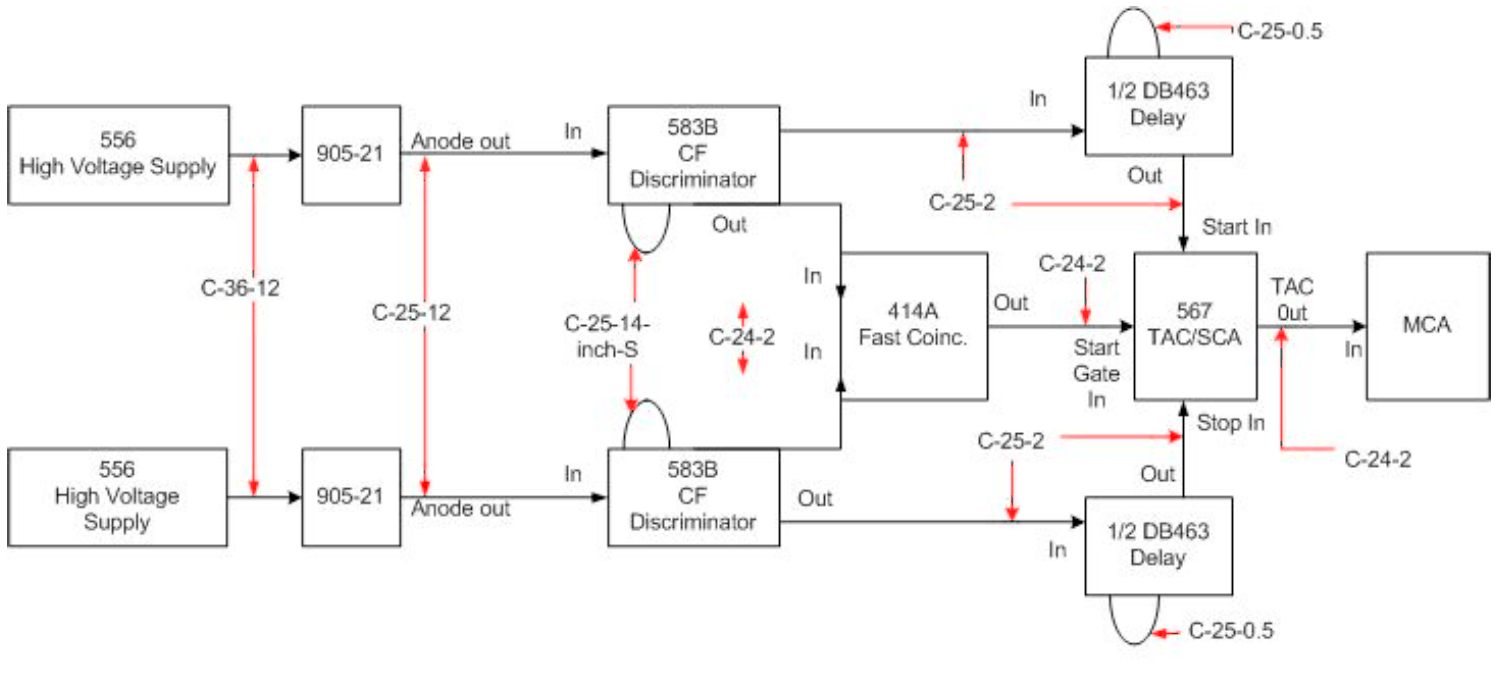
\includegraphics[width=\textwidth]{aufbau.png}
				\caption{Schalt-Schema des Aufbaus für diesen Versuch. Die Bauteile 556 sind jeweils die Detektoren mit den Dynodensystemen. Der MCA ist an einen PC via USB angeschlossen. \cite{EMAUGreifswaldPKO}}
				\label{img:aufbau}
			\end{figure}

			\begin{figure}[h]
				\centering
				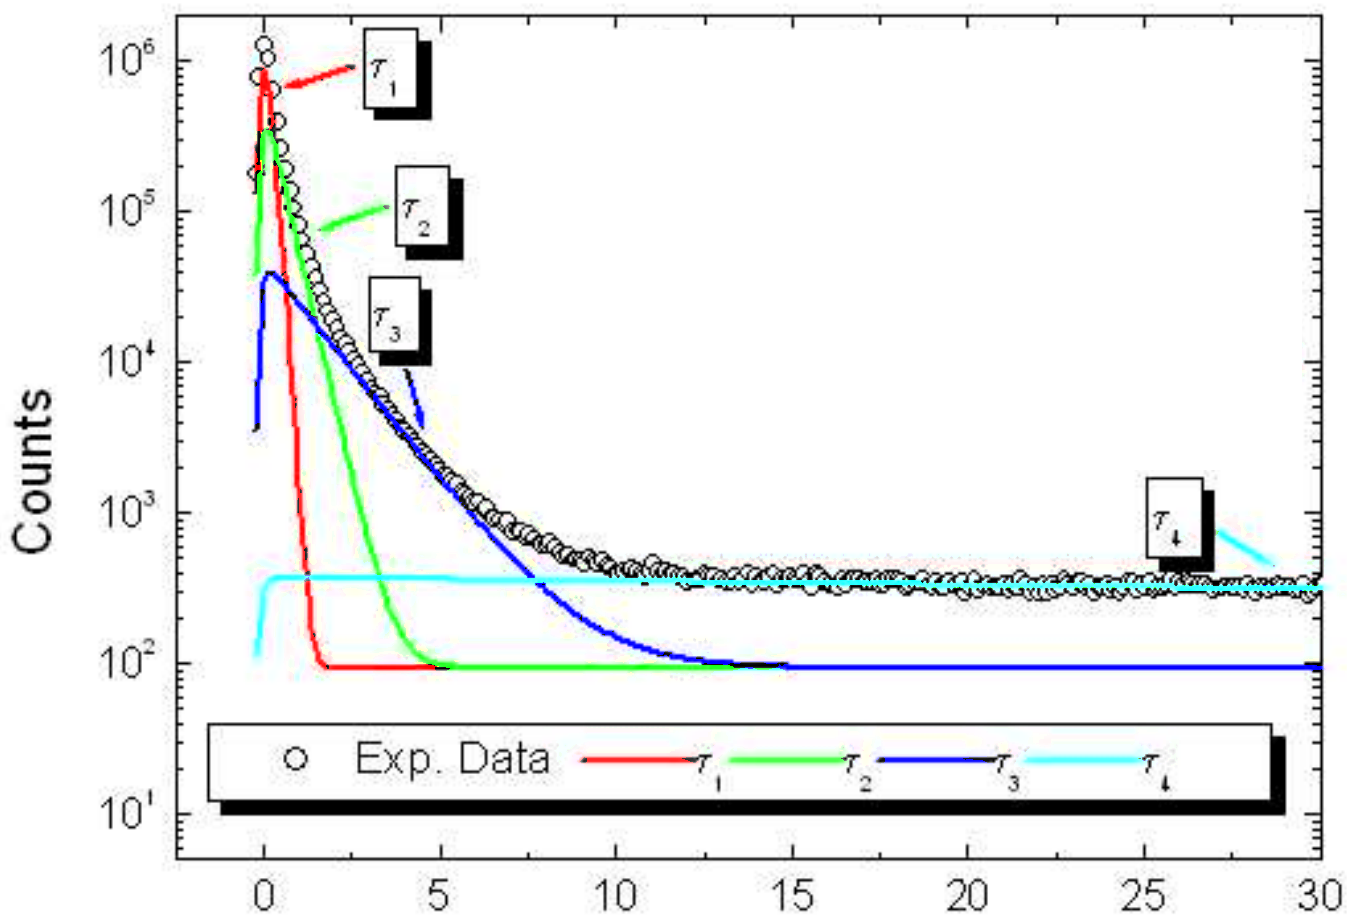
\includegraphics[width=0.6\textwidth]{beispielspektrum.png}
				\caption{Beispiehaftes Spektrum eines Positronen-Lebensdauerspektroskopie mit den unterschiedlichen Lebenszeiten für die verschiedenen "`Lebenswege"' eines $\textbf{e}^+$ $\tau\ix{1}$, $\tau\ix{2}$, \dots \cite{Augsten08}}
				\label{img:beispielspektrum}
			\end{figure}

	\newpage
	\section{Auswertung}
	
	\newpage
	\section{Anhang}

		\bibliography{all.bib}
		\bibliographystyle{plain}

\end{document}